\documentclass[11pt]{article}
\usepackage[review]{acl}
\usepackage{times}
\usepackage{latexsym}
\usepackage[T1]{fontenc}
\usepackage[utf8]{inputenc}
\usepackage{microtype}
\usepackage{amsmath,amssymb,amsthm}
\usepackage{booktabs}
\usepackage{graphicx}
\usepackage{longtable}
\usepackage{stfloats}
\usepackage{placeins}
\usepackage{xcolor}
\usepackage{url}

% In a clean two-column review build, lineno learns column positions through
% the auxiliary file. Keep any first-pass marker inside the gutter, not text.
\ifdefined\linenumbersep
  \setlength{\linenumbersep}{0.2cm}
\fi

\newtheorem{proposition}{Proposition}
\newcommand{\method}{Factor-Contrastive SAE}
\newcommand{\zC}{z_C}
\newcommand{\zS}{z_S}

\title{Factor-Contrastive Sparse Autoencoders:\\Controlled Relations for Stable Multilingual Features}
\author{Anonymous submission}

\begin{document}
\maketitle

\begin{abstract}
Sparse autoencoders can reconstruct activations accurately while assigning a feature to the wrong source of variation: in multilingual data, a feature may follow language rather than meaning. Reconstruction and sparsity specify how compactly an activation is encoded, but not what should remain stable. We introduce the Factor-Contrastive Sparse Autoencoder, which organizes one overcomplete dictionary through reciprocal controlled relations. One sparse route preserves intent while locale changes; the other receives the reversed relation. Matched opposing examples rule out a locale-only shortcut, while blockwise BatchTopK gives both routes independent activity budgets and an ordinary decoder preserves reconstruction. On held-out MASSIVE languages, reciprocal supervision raises intent concept AUC from .701 to .912 and cross-locale stability from .150 to .225 over an architecture-matched reconstruction control. The advantage persists across dictionary widths and transfers across a second multilingual dataset and language-model family. Validation-selected features reach .817 intent purity and .725 reliable coverage. Controlled relations can therefore determine which factor organizes a sparse dictionary without assuming statistical independence or abandoning reconstruction.
\end{abstract}

\section{Introduction}

Sparse autoencoders (SAEs) expose language-model activations as sparse combinations of learned dictionary elements \citep{cunningham2023sparse,gao2024scaling,lieberum2024gemmascope}. Their features are most useful when meaning survives irrelevant changes in wording or language. Yet an SAE trained only for reconstruction may follow whichever correlated pattern best reduces error. Intent and locale, for example, both help reconstruct a multilingual activation, although an intent feature should respond across locales rather than to a locale shared by unrelated utterances. Neither reconstruction nor sparsity expresses this preference. Standard SAE objectives therefore determine capacity and activity without determining which observed factor organizes the learned coordinates; feature quality remains distinct from reconstruction quality \citep{karvonen2025saebench}.

Our central idea is to specify feature organization through relations between examples. For an intent-oriented feature, a positive keeps intent fixed while changing locale; an opposing example keeps locale fixed while changing intent. Locale alone cannot solve this comparison because it favors the opposing example. Reversing the relation defines a locale-oriented route. The two relations state what each route should preserve without assuming statistical independence.

The \method{} applies these relations directly to an overcomplete sparse code. A shared encoder produces intent- and locale-dominant routes, blockwise BatchTopK \citep{bussmann2024batchtopk} reserves a mean activity budget for each, and a linear decoder retains ordinary reconstruction. The relational loss changes feature organization without replacing the dictionary or SAE objective. An architecture-matched control removes only this loss, isolating its effect.

We test concept recovery, stability across held-out languages, reconstruction, and transfer across widths, datasets, and model families. Reciprocal supervision consistently improves feature organization over the exact reconstruction control; Section~\ref{sec:experiments} reports the full comparisons.

\paragraph{Contributions.}
\begin{itemize}
    \item \textbf{Relation-defined factor organization.} Reciprocal matched relations specify which observed factor should dominate each sparse route and exclude a nuisance-only solution.
    \item \textbf{A direct sparse implementation.} Blockwise BatchTopK realizes both routes within one overcomplete dictionary while retaining ordinary reconstruction and an exact capacity-matched control.
    \item \textbf{Feature-level evidence.} Paired experiments across datasets, model families, and dictionary widths connect the relational objective to concept recovery, cross-language stability, and held-out interpretability.
\end{itemize}

\section{Related Work}

\paragraph{Sparse feature learning and evaluation.}
SAEs approximate activations with sparse dictionaries, including large-scale dictionaries across layers and model sizes. Sparsity mechanisms govern how this capacity is used: Top-$k$ fixes per-example activity, BatchTopK fixes mean minibatch activity, and Matryoshka SAEs optimize reconstruction at nested dictionary prefixes \citep{kusupati2022matryoshka,karvonen2025saebench}. Evaluation work separately measures reconstruction and feature quality. These methods control capacity, activity, or reconstruction hierarchy, but leave feature orientation to correlations in the training activations.

\paragraph{Structured sparse autoencoders.}
Relational objectives can structure sparse features beyond reconstruction. T-SAE uses token adjacency to favor temporal consistency \citep{bhalla2026temporal}; geometry-invariant SAEs align features across languages to recover shared reasoning structure \citep{bogdanov2026geometry}. Our target is different: reciprocal relations assign two observed factors to separate activity-controlled routes within one dictionary. The object of evaluation is therefore factor orientation rather than temporal coherence or global alignment.

\paragraph{Contrastive factor isolation.}
Contrastive learning defines representation content through positive and opposing relations \citep{oord2018cpc,zimmermann2021contrastive}. Such structure is necessary because unsupervised factor decomposition is not identifiable without assumptions \citep{locatello2019disentanglement}; controlled transformations can specify what changes and what remains invariant \citep{vonkugelgen2021selfsupervised,cai2023clap}. Factor-Contrastive SAE applies this principle to sparse coordinates: nuisance-matched opposition blocks a nuisance-only solution, and the reversed relation organizes the second route around that nuisance.

\section{Factor-Contrastive Sparse Autoencoder}
\label{sec:method}

The method uses observed relations to determine how a sparse dictionary should organize its features. A relation sampler first states what each route should treat as equivalent and what it must distinguish. A blockwise sparse autoencoder then learns these relations while reconstructing the original activation. Figure~\ref{fig:factor-sae-method} summarizes this two-stage design.

\subsection{Controlled relations define route semantics}

Let $H(x)\in\mathbb{R}^{d}$ be the frozen pooled activation of utterance $x$. Each utterance has an intent $C$ and a locale $S$. The intent route $z_C$ should respond similarly when intent is fixed and locale changes. The locale route $z_S$ should exhibit the reciprocal behavior.

The key comparison is easiest to see from one anchor $x_a$ with intent $c_a$ and locale $s_a$. For $z_C$, the positive keeps the anchor intent but changes locale. The opposing example keeps the anchor locale but changes intent. Formally,
\begin{equation}
\begin{aligned}
C(x_C^+)&=c_a, & S(x_C^+)&\neq s_a,\\
C(x_C^-)&\neq c_a, & S(x_C^-)&=s_a.
\end{aligned}
\label{eq:c-relations}
\end{equation}
This pairing makes the desired distinction explicit: the positive changes the nuisance factor, whereas the opposing example matches it. The $z_S$ route reverses the same pair, using $x_S^+=x_C^-$ and $x_S^-=x_C^+$. It therefore preserves locale while opposing intent.

On MASSIVE, half of the $z_C$ positives are exact translations and half are different semantic IDs with the same intent. Every opposing example has a different intent and the anchor locale. The 50/50 mixture prevents the intent relation from reducing to sentence identity; sampling is balanced over the complete relation set.

\begin{proposition}
If negatives for $z_C$ are matched on $S$, a representation that depends only on $S$ cannot rank $x_C^+$ above $x_C^-$ for every relation.
\label{prop:matched-shortcut}
\end{proposition}
An $S$-only representation maps $x_a$ and $x_C^-$ to the same value, making the opposing similarity maximal, while $x_C^+$ changes $S$. It therefore cannot satisfy every $z_C$ relation. Appendix~\ref{app:shortcut-proof} gives the formal argument; the reciprocal construction gives the same protection to $z_S$.

\subsection{Learning the relations in a sparse dictionary}

The relations supervise sparse features directly rather than first creating a dense bottleneck. A shared encoder maps $H(x)$ into one overcomplete pre-activation vector and assigns disjoint coordinates to the two routes:
\begin{equation}
\begin{aligned}
a(x)&=W_{\mathrm{enc}}H(x)+b_{\mathrm{enc}},\\
a&=[a_C;a_S]\in\mathbb{R}^{m}.
\end{aligned}
\end{equation}
A single global sparsity budget could allow one route to consume nearly all active features. We instead apply BatchTopK separately to the two blocks \citep{bussmann2024batchtopk}:
\begin{equation}
\begin{aligned}
z_C&=\operatorname{BatchTopK}_{k_C}(a_C),\\
z_S&=\operatorname{BatchTopK}_{k_S}(a_S).
\end{aligned}
\label{eq:sparse-routes}
\end{equation}
For a batch of $B$ examples, the blocks retain their largest $Bk_C$ and $Bk_S$ positive activations. Each example may use more or fewer features, but each route receives a guaranteed mean activity budget. Training-calibrated thresholds make test-time inference independent of batch composition.

The exact blockwise control uses the same encoder, route widths, activity budgets, decoder, and optimizer but removes both relational losses. Its difference from the proposed model therefore isolates the effect of controlled relations rather than the block allocation.

The decoder reconstructs the original activation from the concatenated code:
\begin{equation}
\widehat H=W_{\mathrm{dec}}[z_C;z_S]+b_{\mathrm{dec}},\qquad
\mathcal{L}_{\mathrm{rec}}=\lVert H-\widehat H\rVert_2^2.
\label{eq:reconstruction}
\end{equation}
Following standard Top-$k$ SAE training \citep{gao2024scaling}, decoder columns are normalized after every optimization step.

\begin{figure*}[t]
\centering
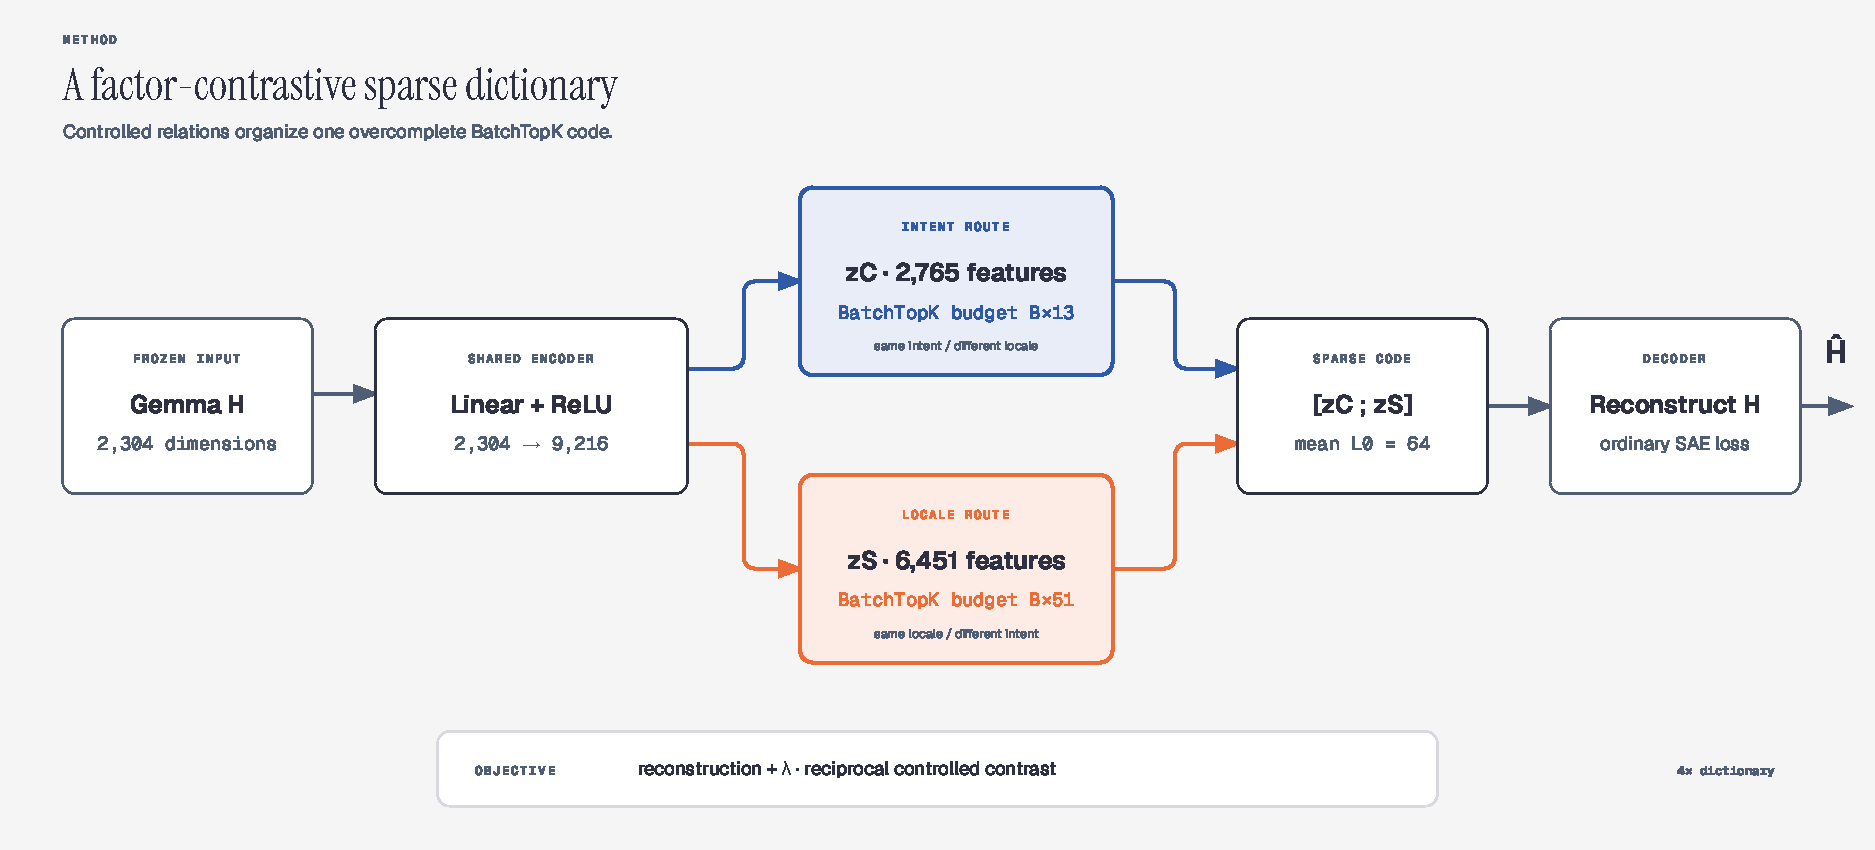
\includegraphics[width=\textwidth]{Figures/factor_sae_figure1_method.pdf}
\caption{Factor-contrastive sparse autoencoder. A shared encoder maps frozen activations into one overcomplete dictionary. Blockwise BatchTopK assigns separate activity budgets to the intent- and locale-dominant routes; reciprocal controlled relations organize the routes while an ordinary linear decoder reconstructs the input activation.}
\label{fig:factor-sae-method}
\end{figure*}

The relational objective asks each route to rank its positive above its matched opposing example. For route $r\in\{C,S\}$, let $\bar z_r=z_r/\lVert z_r\rVert_2$, $u_r^+=\bar z_r(x_a)^\top\bar z_r(x_r^+)$, and $u_r^-=\bar z_r(x_a)^\top\bar z_r(x_r^-)$. We use the standard contrastive softmax form \citep{oord2018cpc,zimmermann2021contrastive}:
\begin{equation}
\begin{aligned}
\mathcal{L}_r&=-\log\frac{\exp(u_r^+/\tau)}
{\exp(u_r^+/\tau)+\exp(u_r^-/\tau)},\\
\mathcal{L}&=\mathcal{L}_{\mathrm{rec}}
+\frac{\lambda}{2}(\mathcal{L}_C+\mathcal{L}_S).
\end{aligned}
\label{eq:route-loss}
\end{equation}
The first term preserves ordinary SAE reconstruction; the two relational terms determine which factor organizes each route. No adversarial, orthogonality, independence, prototype, or swap-training term is used.

The main model uses a fourfold dictionary; an eightfold version tests sparse-width sensitivity. Appendix~\ref{app:protocol} gives the exact route dimensions and activity budgets. Complementarity is evaluated from the learned routes rather than imposed by an auxiliary constraint.

\section{Experimental Evaluation}
\label{sec:experiments}

The experiments ask four questions. Do controlled relations improve intent-oriented features over an identical reconstruction-only model? Do these gains remain when reconstruction and activity are measured? Are the learned features stable and interpretable across held-out locales? Finally, do the conclusions transfer across sparse widths, datasets, and model families? Appendix~\ref{app:protocol} contains the complete protocol and configuration.

\subsection{Experimental design}

\paragraph{Models and data.}
The main experiment uses masked-mean hidden-state-8 activations from Gemma~2~2B \citep{gemmateam2024gemma2} on MASSIVE \citep{fitzgerald2023massive}. Training contains 10,343 semantic IDs from 49 locales; validation contains 1,149 disjoint IDs. The final test set contains 2,968 untouched IDs, each observed in Arabic and Chinese. Transfer experiments use MTOP \citep{li2021mtop} and Pythia-160M \citep{biderman2023pythia}.

\paragraph{Fair comparisons.}
We compare raw $H$, global BatchTopK, the exact blockwise reconstruction control, Matryoshka SAE reconstruction, one-sided supervision, and a validation-selected triplet loss \citep{schroff2015facenet}. Learned comparisons share their inputs, dictionary capacity, activity, initialization, batches, optimizer, epochs, and paired seeds. Thus the blockwise control differs from our model only in the relational objective.

\paragraph{What a successful route should do.}
A useful $z_C$ feature should identify an intent, activate consistently for its translations, and reveal less locale information. We measure these properties with intent concept AUC, Arabic--Chinese activation correlation, and a locale probe. Intent- and locale-oriented feature fractions show which factor dominates the active dictionary. The reciprocal diagnostics ask whether $z_S$ retains locale while suppressing intent.

Intent concept AUC is the mean one-vs-rest held-out AUC \citep{fawcett2006roc} of one validation-selected coordinate per intent. Stability is the mean Pearson correlation \citep{pearson1895regression} between paired Arabic and Chinese activations. Balanced logistic probes \citep{cox1958regression} measure locale in $z_C$ and locale or intent in $z_S$. We report reconstruction as fraction of variance explained (FVE) and sparsity as the observed number of active features.

Every method uses the same feature-selection split, probe split, test split, and evaluator. Features are selected only on validation data, and all comparison tables report mean $\pm$ standard deviation over three paired seeds. Appendix~\ref{app:protocol} defines feature activity, orientation, probe selection, and bootstrap estimation.

\paragraph{Validation before testing.}
Validation selects the reciprocal binary objective and triplet margin $m=.2$ from $\{.1,.2,.4\}$. The Arabic--Chinese test activations are then evaluated once. No test result selects a model, feature, intent, or displayed example.

\subsection{Controlled relations reorganize the routes}

\begin{table*}[t]
\centering
\caption{MASSIVE results on held-out Arabic and Chinese. Blockwise methods are evaluated on $z_C$ in the primary columns. Lower locale probe, locale-oriented fraction, and $z_S$ intent probe are better.}
\label{tab:factor-sae-test}
\resizebox{\textwidth}{!}{%
\begin{tabular}{lrrrrrrrr}
\toprule
Method & Intent AUC $\uparrow$ & Stability $\uparrow$ & Locale probe $\downarrow$ & Intent frac. $\uparrow$ & Locale frac. $\downarrow$ & $z_S$ locale $\uparrow$ & $z_S$ intent $\downarrow$ & FVE $\uparrow$ \\
\midrule
Raw $H$ & .7703 & .3013 & .9997 & .1159 & .7409 & -- & -- & -- \\
BatchTopK SAE & $.7940\pm.0014$ & $.1278\pm.0011$ & $.9871\pm.0048$ & $.4579\pm.0026$ & $.4723\pm.0030$ & -- & -- & $.6618\pm.0017$ \\
Blockwise control & $.7007\pm.0109$ & $.1501\pm.0080$ & $.9665\pm.0106$ & $.4830\pm.0122$ & $.4465\pm.0122$ & $.9878\pm.0014$ & $.4798\pm.0151$ & $.6627\pm.0002$ \\
Matryoshka SAE & $.8352\pm.0150$ & $.1385\pm.0017$ & $.9821\pm.0009$ & $.4686\pm.0018$ & $.4652\pm.0033$ & -- & -- & $.6482\pm.0014$ \\
One-sided factor SAE & $\mathbf{.9165\pm.0083}$ & $.1813\pm.0061$ & $.8969\pm.0143$ & $.6923\pm.0198$ & $.2427\pm.0163$ & $.9861\pm.0029$ & $.4679\pm.0004$ & $.6415\pm.0015$ \\
\textbf{Reciprocal factor SAE (ours)} & $.9124\pm.0027$ & $\mathbf{.2248\pm.0035}$ & $\mathbf{.8944\pm.0034}$ & $\mathbf{.7864\pm.0144}$ & $\mathbf{.1646\pm.0065}$ & $\mathbf{.9925\pm.0008}$ & $.3892\pm.0079$ & $.6098\pm.0011$ \\
Triplet, $m=.2$ & $.9063\pm.0190$ & $.1983\pm.0029$ & $.9096\pm.0049$ & $.7274\pm.0013$ & $.2043\pm.0011$ & $.9916\pm.0029$ & $\mathbf{.3818\pm.0171}$ & $\mathbf{.6427\pm.0012}$ \\
\bottomrule
\end{tabular}%
}
\end{table*}

Controlled relations reorganize both routes in the intended direction. Against the exact blockwise control, our $z_C$ raises intent AUC from .7007 to .9124 and stability from .1501 to .2248. Its intent-oriented feature fraction rises from .4830 to .7864, while its locale-oriented fraction falls from .4465 to .1646. The reciprocal $z_S$ route reaches .9925 locale accuracy and reduces intent leakage from .4798 to .3892. Because the control removes only the relational losses, these changes isolate relational supervision.

The same conclusion holds against the standard sparse alternatives. Relative to global BatchTopK, intent AUC increases by .1185 and stability by .0970; relative to Matryoshka, the gains are .0772 and .0863. The complete-route intent probe remains close to global BatchTopK (.4625 versus .4680), indicating that stronger organization in $z_C$ does not remove intent from the joint sparse code.

Raw $H$ is a dense reference, not a sparse baseline. Locale is almost perfectly decoded from it (.9997), and 74.1\% of its coordinates are locale-oriented. In contrast, the learned $z_C$ is sparse and overcomplete, with 78.6\% intent-oriented and 16.5\% locale-oriented active features. The result is therefore a change in feature organization, not simply the presence of intent somewhere in the representation.

\subsection{Reconstruction and activity}

The factor gains are obtained at matched sparse activity with a moderate reconstruction trade-off. All models train at mean $L_0=64$, and their frozen thresholds produce similar held-out activity: $104.46\pm.07$ for ours, $105.99\pm.81$ for the exact control, and $107.16\pm.91$ for global BatchTopK. Reconstruction FVE is .6098 for ours and .6627 for the exact control, an 8.0\% relative difference.

Held-out $L_0$ exceeds the training budget because test examples use thresholds calibrated on seen locales rather than a newly computed test-batch budget. Since ours and the controls have nearly identical held-out activity, the AUC and stability gains cannot be explained by a larger test-time code. Appendix~\ref{app:protocol} gives the shared thresholding and reconstruction protocol.

\subsection{Cross-locale feature consistency}

\begin{figure*}[t]
\centering
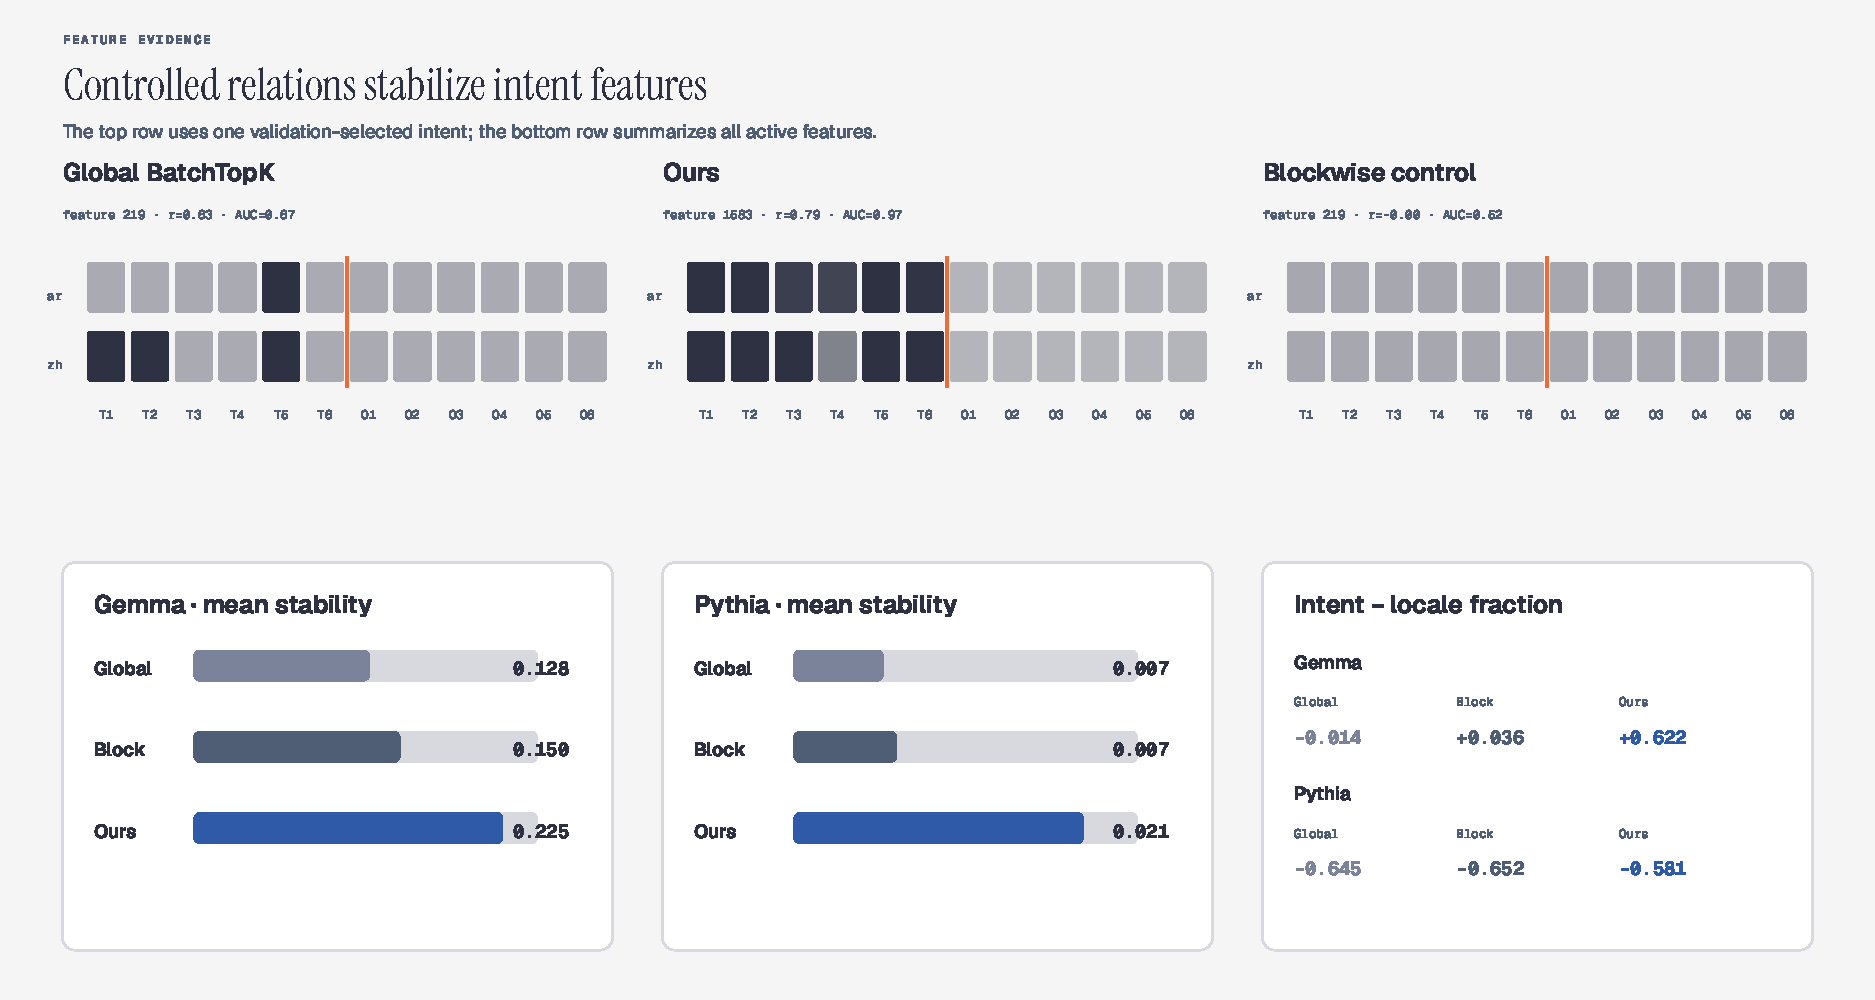
\includegraphics[width=\textwidth]{Figures/factor_sae_figure3_stability.pdf}
\caption{Controlled relations stabilize intent features. Top: each Gemma method selects its own feature for the same validation-selected intent; T1--T6 and O1--O6 are held-out target- and comparison-intent semantic IDs in Arabic and Chinese. Bottom: three-seed all-feature stability and intent-minus-locale orientation for Gemma and Pythia.}
\label{fig:factor-feature-stability}
\end{figure*}

Figure~\ref{fig:factor-feature-stability} shows what the aggregate stability gain looks like for one intent feature. The reciprocal feature responds similarly to Arabic and Chinese instances of its target intent, reaching held-out AUC .97 and stability .79. The blockwise-control feature for the same validation-selected intent reaches AUC .52 and approximately zero stability. The dictionary-wide averages give the same ordering for both Gemma (.2248 versus .1501) and Pythia (.0211 versus .0075).

Feature and intent selection use disjoint validation splits; held-out activations are never used to choose the example. Test labels only identify the six deterministically ordered target and comparison instances after selection. The complete selection rule appears in Appendix~\ref{app:protocol}.

\subsection{Intent-feature interpretability}

\begin{table*}[t]
\centering
\caption{Validation-selected intent features on held-out MASSIVE Arabic and Chinese. Purity and reliable coverage use 46 intents with at least 20 test semantic IDs; stability covers all 58 intents.}
\label{tab:factor-feature-interpretability}
\resizebox{.92\textwidth}{!}{%
\begin{tabular}{lrrrr}
\toprule
Method & Purity@20 $\uparrow$ & Reliable coverage $\uparrow$ & Selected stability $\uparrow$ & Top-ID overlap $\downarrow$ \\
\midrule
Global BatchTopK & $.653\pm.020$ & $.370\pm.022$ & $.457\pm.004$ & $.0025\pm.0005$ \\
Blockwise control & $.581\pm.068$ & $.341\pm.091$ & $.375\pm.040$ & $.0034\pm.0012$ \\
\textbf{Reciprocal factor SAE (ours)} & $\mathbf{.817\pm.012}$ & $\mathbf{.725\pm.045}$ & $\mathbf{.563\pm.003}$ & $\mathbf{.0022\pm.0001}$ \\
\bottomrule
\end{tabular}%
}
\end{table*}

The stable features are also more interpretable. Reciprocal supervision raises Purity@20 by .236 and reliable coverage by .384 over the exact blockwise control. Its near-zero top-ID overlap indicates that different intent features retrieve distinct examples rather than the same globally active utterances.

Purity ranks unique semantic IDs by the larger activation across their Arabic and Chinese translations. The calculation covers the 46 intents with at least 20 held-out IDs; reliable coverage is the fraction whose selected feature reaches at least .8 purity. Selected-feature stability covers all 58 intents.

The normalized locale entropy of our top activation sets is .633, close to global BatchTopK (.636), so high purity does not come from retrieving only one held-out locale. Appendix~\ref{app:feature-examples} provides the complete 58-intent catalogue and qualitative examples.

\begin{figure*}[t]
\centering
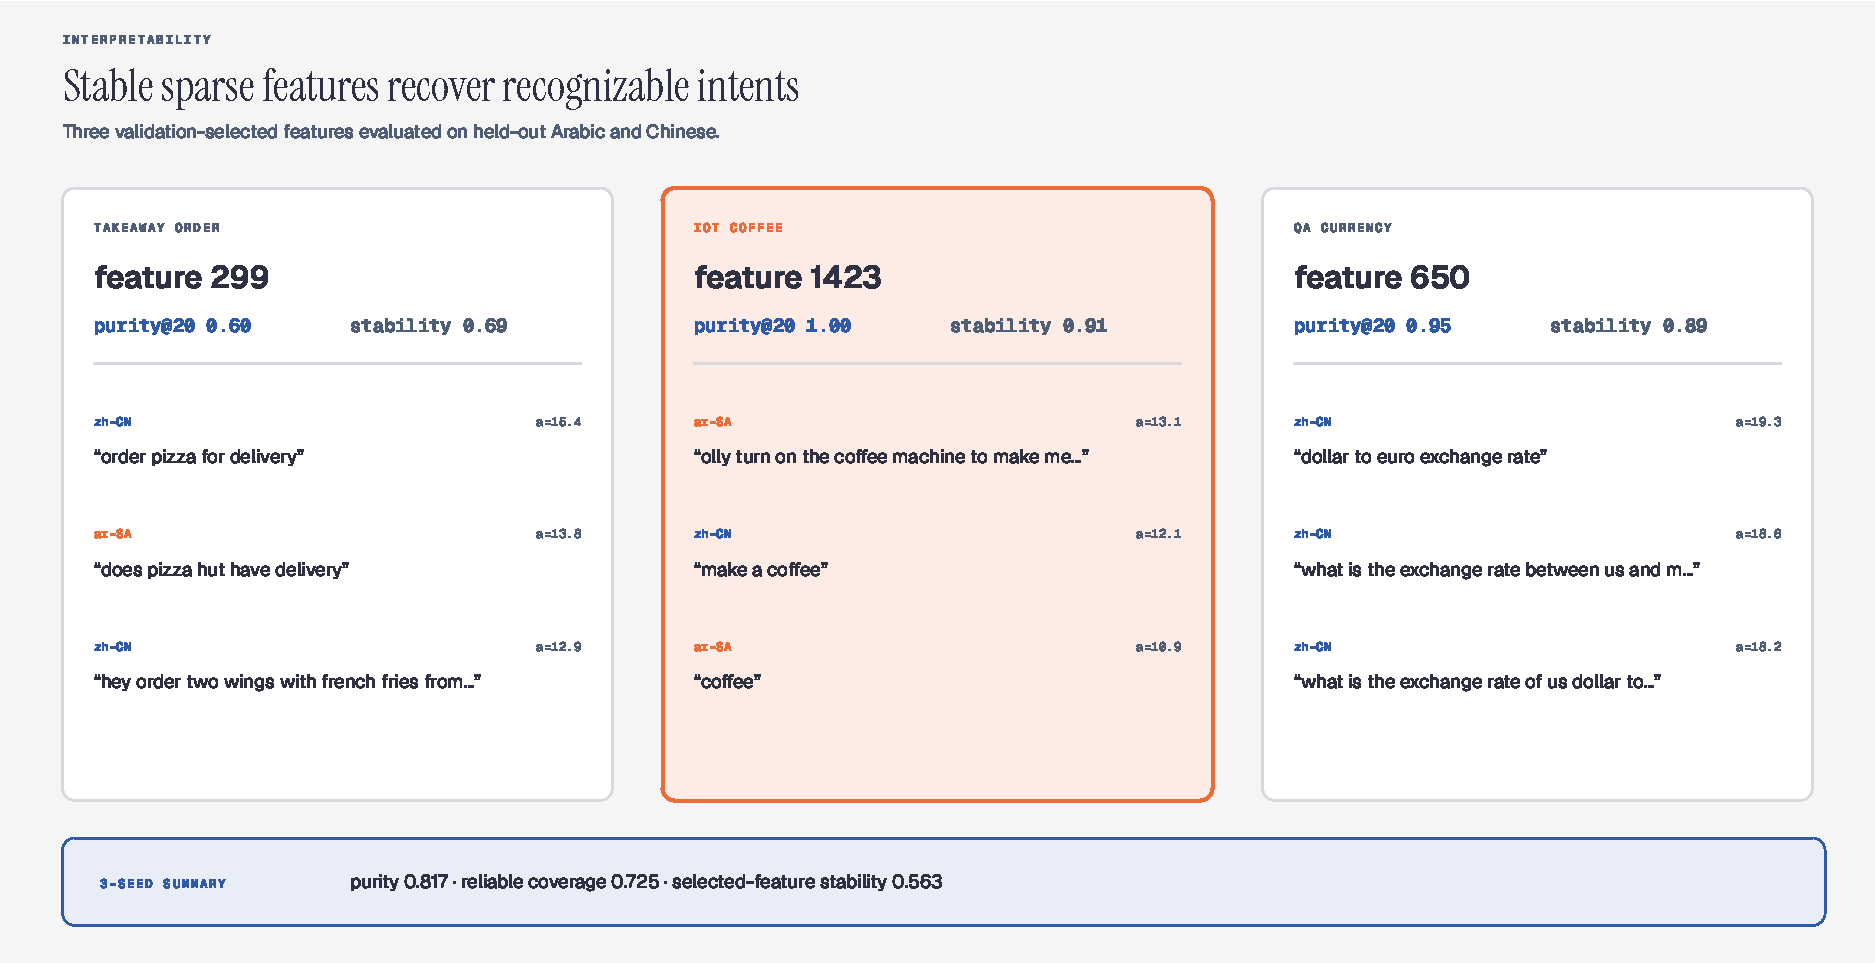
\includegraphics[width=\textwidth]{Figures/factor_sae_figure4_examples.pdf}
\caption{Validation-selected sparse features recover recognizable intent concepts on held-out Arabic and Chinese. The cards show representative high-activation examples for three intent features; selection uses validation data only, while purity and stability are measured on the held-out locales.}
\label{fig:factor-sae-examples}
\end{figure*}

The complete representative-seed catalogue contains all 58 intent features, including feature IDs, purity, stability, held-out AUC, and activity support (Appendix~\ref{app:feature-examples}). The machine-readable catalogue extends this evaluation to all three methods and seeds.

\subsection{Robustness, transfer, and ablations}

\begin{figure*}[t]
\centering
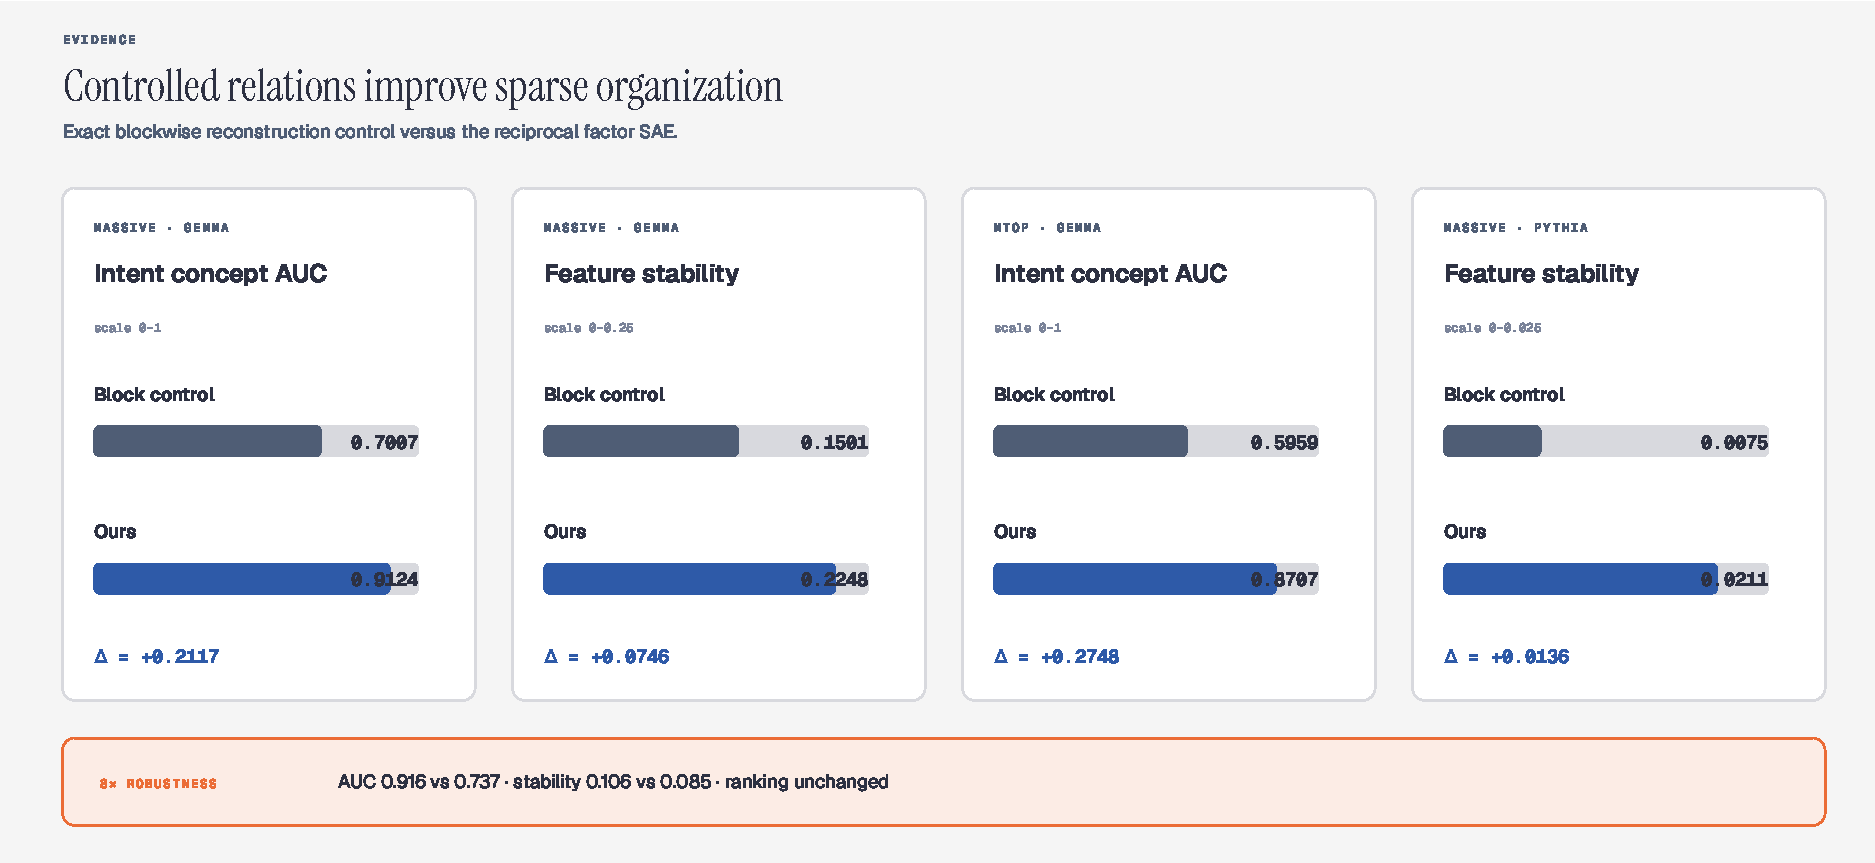
\includegraphics[width=\textwidth]{Figures/factor_sae_figure2_evidence.pdf}
\caption{The controlled-relation advantage transfers across datasets and model families and persists at eightfold width. All panels compare against the exact blockwise reconstruction control; the Pythia table and complete protocol are in Appendix~\ref{app:transfer-tables}.}
\label{fig:factor-sae-evidence}
\end{figure*}

The controlled-relation advantage persists when the dictionary is widened, exact translation IDs are removed, or the activation model is changed. Figure~\ref{fig:factor-sae-evidence} summarizes these three tests; the tables below and Appendix~\ref{app:transfer-tables} give the full results.

\begin{table*}[t]
\centering
\caption{MASSIVE width robustness. Dictionary width and activity double together from $4\times$/$L_0=64$ to $8\times$/$L_0=128$.}
\label{tab:factor-sae-width}
\resizebox{.94\textwidth}{!}{%
\begin{tabular}{llrrrrrr}
\toprule
Width & Method & AUC $\uparrow$ & Stability $\uparrow$ & Locale probe $\downarrow$ & Intent frac. $\uparrow$ & Locale frac. $\downarrow$ & FVE $\uparrow$ \\
\midrule
$4\times$ & Global BatchTopK & .7940 & .1278 & .9871 & .4579 & .4723 & .6618 \\
$4\times$ & Blockwise control & .7007 & .1501 & .9665 & .4830 & .4465 & .6627 \\
$4\times$ & \textbf{Ours} & \textbf{.9124} & \textbf{.2248} & \textbf{.8944} & \textbf{.7864} & \textbf{.1646} & .6098 \\
\midrule
$8\times$ & Global BatchTopK & .8094 & .0797 & .9908 & .4408 & .4637 & .7152 \\
$8\times$ & Blockwise control & .7373 & .0847 & .9760 & .4494 & .4562 & .7154 \\
$8\times$ & \textbf{Ours} & \textbf{.9156} & \textbf{.1063} & \textbf{.9397} & \textbf{.6708} & \textbf{.2530} & .6705 \\
\bottomrule
\end{tabular}%
}
\end{table*}

Doubling dictionary width and activity preserves the main ordering. At eightfold width, reciprocal supervision improves AUC by .1783 and stability by 25.6\% over the exact control. FVE remains within 6.3\% of the control, and intent AUC is nearly unchanged across widths (.9124 and .9156).

\begin{table*}[t]
\centering
\caption{MTOP transfer to held-out Hindi and Thai (three paired seeds). Lower language probe and $z_S$ intent are better.}
\label{tab:factor-sae-mtop}
\resizebox{\textwidth}{!}{%
\begin{tabular}{lrrrrrrr}
\toprule
Method & AUC $\uparrow$ & Stability $\uparrow$ & Margin $\uparrow$ & Lang. probe $\downarrow$ & R@1 $\uparrow$ & $z_S$ lang. $\uparrow$ & $z_S$ intent $\downarrow$ \\
\midrule
Raw $H$ & .7859 & .5443 & -.0724 & 1.0000 & .7998 & -- & -- \\
Global BatchTopK & $.6529\pm.0038$ & $.3605\pm.0023$ & $.0341\pm.0024$ & $.9837\pm.0020$ & $.7010\pm.0062$ & -- & -- \\
Blockwise control & $.5959\pm.0186$ & $.3701\pm.0119$ & $.0228\pm.0100$ & $.9416\pm.0050$ & $.4900\pm.0391$ & $.9795\pm.0027$ & $.5071\pm.0140$ \\
\textbf{Ours} & $\mathbf{.8707\pm.0017}$ & $\mathbf{.4978\pm.0153}$ & $\mathbf{.3441\pm.0105}$ & $\mathbf{.9278\pm.0034}$ & $\mathbf{.7809\pm.0166}$ & $\mathbf{.9857\pm.0035}$ & $\mathbf{.4639\pm.0062}$ \\
\bottomrule
\end{tabular}%
}
\end{table*}

MTOP tests whether exact translations are necessary. Training uses German, English, Spanish, and French, while Hindi and Thai are held out. Because MTOP has no parallel semantic IDs, stability compares each feature's 50-intent activation profile across the two test languages. Reciprocal supervision improves AUC by .2748, stability by .1277, relation margin by .3214, and retrieval R@1 by .2910 over the exact blockwise control. The same objective therefore transfers without exact translations or dataset-specific architectural changes.

Pythia-160M tests a different activation geometry. Reciprocal supervision raises stability from .0075 to .0211 and improves relation margin by .4797 over the blockwise control, with the same direction in all three paired seeds. It also improves feature orientation, locale leakage, and the opposing route. The absolute AUC change is small in this weaker activation space; stability, margin, and route organization provide the transfer evidence. No Pythia-specific loss or sparsity setting is introduced.

The component ablations support reciprocal binary supervision. One-sided training attains slightly higher intent AUC (.9165 versus .9124), but reciprocal training improves stability by .0434, raises the intent-oriented fraction by .0941, lowers the locale-oriented fraction by .0781, and reduces $z_S$ intent leakage by .0787. The triplet loss retains more reconstruction FVE (.6427 versus .6098) but is lower on AUC, stability, locale leakage, and feature orientation. These results motivate the reciprocal binary objective used throughout the transfer experiments.


\section{Discussion and Conclusions}

\paragraph{Controlled relations change feature organization.}
The exact blockwise control is the key comparison because it shares every architectural and optimization choice with the proposed model. Its gap to the reciprocal model therefore measures the effect of the controlled relations. On MASSIVE, reciprocal supervision increases intent AUC, cross-locale stability, and the intent-oriented feature fraction while decreasing the locale-oriented fraction. The reciprocal $z_S$ result shows that this change is not obtained by simply suppressing the second route: the opposing block retains locale and loses intent information in the intended direction.

\paragraph{The result is not tied to one sparse scale.}
The same ordering holds when dictionary width and activity are doubled. Absolute coordinate-level stability decreases at eightfold width because evidence is distributed across more active coordinates, but the relational advantage remains and intent AUC is unchanged. The fourfold model is therefore the compact operating point rather than a uniquely favorable width.

\paragraph{Relational supervision transfers.}
MTOP removes the exact translation identifiers available in MASSIVE, yet same-intent/different-language relations improve AUC, margin, retrieval, and stability on held-out Hindi and Thai. Pythia-160M changes activation dimensionality and model family while preserving the sparse capacity and objective. The consistent direction indicates that the effect follows the controlled relations rather than one model-specific activation geometry.

\paragraph{Scope and conclusion.}
The method requires observed factors from which controlled relations can be constructed; the present evidence concerns multilingual intent and language. It targets factor-dominant routes rather than coordinate-wise statistical independence. Within this setting, the results support a simple design principle: when a desired invariance can be expressed as a matched relation, it can be imposed directly on sparse feature learning while retaining the standard reconstruction objective.

\bibliography{references}

\clearpage
\onecolumn
\appendix
\section{Frozen Experimental Protocol}
\label{app:protocol}

\subsection{MASSIVE split and relation audit}

The MASSIVE split is fixed by semantic ID. Representation training contains 10,343 IDs, validation contains 1,149 disjoint IDs, and the untouched Arabic--Chinese test set contains 2,968 IDs. Feature selection uses 5,220 balanced validation rows spanning all 58 intents and 49 seen locales; its fit and scoring semantic IDs are disjoint. Probe fitting uses 5,800 balanced training rows. The canonical manifest hash is \texttt{6c33455d91ccd15fc6054c3f077cb2393f387ab136db71fcea76f581d7344439}.

For $z_C$, half of sampled positives are exact translations and half use a different semantic ID with the same intent. Every opposing example has a different intent and the anchor locale. The aggregate schedule is exactly balanced; intents with only one semantic ID necessarily contribute exact translations, and eligible anchors from other intents compensate with different-ID positives. The $z_S$ route reverses the assignments.

\subsection{Deterministic sampler and evaluator}

The sampler and evaluator follow one frozen sequence for every learned comparison:
\begin{enumerate}
\item sample an anchor from the fixed training-ID manifest;
\item with probability .5, choose its exact translation as the $z_C$ positive; otherwise choose a different semantic ID with the same intent in a different locale;
\item choose the $z_C$ opposing example with a different intent in the anchor locale, and reverse these assignments for $z_S$;
\item apply global or blockwise BatchTopK according to the comparison while keeping the same batch order and mean activity budget;
\item select one coordinate per intent using only the validation fit split, score selection on the disjoint validation score split, and freeze the selected coordinates;
\item evaluate the frozen model and selected coordinates once on the held-out locale test split.
\end{enumerate}
Batch ordering and relation sampling use separate seeded random generators. Ties in ranking metrics follow stable row order, and every method uses the same active-feature, variance-floor, probe, and bootstrap implementations.

\subsection{Shortcut proposition}
\label{app:shortcut-proof}

Let similarity be cosine similarity and suppose $z_C(x)=f(S(x))$. Since $S(x_a)=S(x_C^-)$, $z_C(x_a)=z_C(x_C^-)$ and therefore $u_C^-=1$ whenever the code is nonzero. Cosine similarity is at most one, so $u_C^+>u_C^-$ is impossible. Consequently, an $S$-only representation cannot satisfy the strict ranking required by every matched relation. The argument does not require statistical independence between $C$ and $S$; it uses only the matched construction in Equation~\ref{eq:c-relations}.

\subsection{Metric definitions}

Intent concept AUC is the mean one-vs-rest held-out AUC of one validation-selected coordinate per intent. Cross-locale stability is the mean Pearson correlation of paired Arabic--Chinese feature activations across active coordinates. An intent-oriented feature has intent selectivity greater than $1.1$ times locale selectivity; locale orientation is defined symmetrically. Locale leakage is balanced locale-probe accuracy on $z_C$. Opposing-route diagnostics report locale accuracy and intent balanced accuracy \citep{brodersen2010balanced} on $z_S$. Probe coordinates are selected by training-only one-way ANOVA \citep{fisher1925statistical} before the standardized logistic model is fitted.

Interpretability selects one feature per intent on the disjoint validation fit split. Held-out Arabic and Chinese translations are merged by semantic ID using the larger activation, then ranked. Purity@20 is the fraction of the first 20 unique IDs carrying the selected intent. Reliable coverage is the fraction of eligible intents whose purity is at least .8. The headline calculation contains the 46 intents with at least 20 held-out IDs.

All feature metrics use variance floor $10^{-12}$, activation threshold $10^{-8}$, and minimum activity rate $10^{-3}$. Bootstrap confidence intervals use 10,000 resamples \citep{efron1993bootstrap}. Tables report mean $\pm$ standard deviation over seeds 20260827, 20260828, and 20260829.

\subsection{Training configuration}

All learned comparisons use AdamW \citep{loshchilov2019adamw}. Table~\ref{tab:appendix-training} gives the exact dimensions, route budgets, optimization settings, and training duration for the main experiment.

\begin{table}[h]
\centering
\caption{Frozen fourfold MASSIVE configuration.}
\label{tab:appendix-training}
\begin{tabular}{lr}
\toprule
Choice & Value \\
\midrule
Activation source & Gemma 2 2B, hidden state 8 \\
Input / dictionary width & 2,304 / 9,216 \\
$z_C / z_S$ widths & 2,765 / 6,451 \\
BatchTopK budgets & $13B / 51B$ \\
Mean training $L_0$ & 64 \\
Batch size / epochs & 128 / 30 \\
Optimizer / learning rate & AdamW / $10^{-4}$ \\
Temperature $\tau$ / weight $\lambda$ & .07 / 1 \\
\bottomrule
\end{tabular}
\end{table}

At eightfold width, the dictionary contains 18,432 coordinates and uses budgets $26B/102B$, preserving route proportions and active fraction. MTOP uses the main fourfold configuration. Pythia-160M uses 768-dimensional hidden-state-8 activations while retaining the 9,216-coordinate dictionary and $13B/51B$ budgets. Training was performed on a single NVIDIA RTX 3090 with 24GB memory.

\subsection{Layer sensitivity}

The main experiments use Gemma hidden state 8. To test whether the result depends on that choice, we repeat the decisive paired comparison at hidden states 4, 8, 16, and 24. Each layer receives its own training-set normalization, and the proposed model and exact blockwise control start from the same fresh initialization. The manifest, sampler, dictionary, activity budgets, optimizer, training duration, and evaluator are otherwise unchanged. This appendix experiment uses seed 20260827; the main hidden-state-8 result in Table~\ref{tab:factor-sae-test} remains the three-seed estimate.

\begin{table}[h]
\centering
\caption{Gemma layer sensitivity. Each entry is exact blockwise control / ours from a paired run. The proposed relations improve intent AUC and cross-locale stability and reduce locale-probe accuracy at all four layers.}
\label{tab:layer-sensitivity}
\resizebox{\textwidth}{!}{%
\begin{tabular}{rrrrrr}
\toprule
Hidden state & Intent AUC $\uparrow$ & Stability $\uparrow$ & Locale probe $\downarrow$ & FVE $\uparrow$ & Held-out $L_0$ \\
\midrule
4  & .6225 / \textbf{.8989} & .0277 / \textbf{.0594} & .9720 / \textbf{.9053} & .4879 / .4367 & 109.13 / 105.03 \\
8  & .7132 / \textbf{.9097} & .1509 / \textbf{.2184} & .9639 / \textbf{.8908} & .6631 / .6098 & 107.57 / 105.45 \\
16 & .6847 / \textbf{.8956} & .1613 / \textbf{.2223} & .9879 / \textbf{.9464} & .7222 / .6680 & 117.40 / 118.60 \\
24 & .6771 / \textbf{.9173} & .0857 / \textbf{.1463} & .9808 / \textbf{.9609} & .6392 / .6030 & 139.18 / 132.72 \\
\bottomrule
\end{tabular}%
}
\end{table}

The strongest absolute AUC occurs at hidden state 24, whereas hidden state 8 gives the lowest locale probe and nearly the highest stability. More importantly, the paired direction is invariant to layer choice: AUC improves by .1965--.2764, stability by .0317--.0675, and locale-probe accuracy falls by .0199--.0731. The reconstruction cost is modest and consistent, with FVE decreasing by .0362--.0542.

\subsection{Software and computation}

\begin{table}[h]
\centering
\caption{Frozen software and execution environment. Versions are taken from the submitted \texttt{uv.lock}.}
\label{tab:software-compute}
\begin{tabular}{ll}
\toprule
Component & Version or setting \\
\midrule
Python & $\geq 3.12,<3.14$ \\
PyTorch / CUDA build & 2.7.1 / cu128 \\
Transformers / Datasets & 5.15.1 / 5.0.1 \\
NumPy / pandas & 2.5.2 / 3.0.5 \\
scikit-learn / Accelerate & 1.9.0 / 1.14.0 \\
SAE Lens & 6.49.1 \\
Hardware & NVIDIA RTX 3090, 24GB \\
Gemma extraction & bfloat16 model, float32 pooled arrays \\
Pythia extraction & float16 model, float32 pooled arrays \\
Tokenization / pooling & 128 tokens / masked non-padding mean \\
\bottomrule
\end{tabular}
\end{table}

The fourfold Gemma/MTOP SAE has 42,478,848 trainable encoder/decoder parameters, the eightfold model has 84,955,392, and the Pythia model has 14,165,760. The final study comprises 53 thirty-epoch training runs: 18 MASSIVE main comparisons, nine eightfold runs, nine MTOP runs, nine Pythia runs, and eight paired layer-sensitivity runs, in addition to the frozen validation candidates. Saved checkpoints are approximately 170MB, 340MB, and 56.7MB for the fourfold Gemma/MTOP, eightfold Gemma, and Pythia configurations, respectively.

\section{Comparison and Selection Details}

Global BatchTopK uses one dictionary and a global $64B$ activity budget. The exact blockwise control has the proposed encoder, decoder, 30/70 route widths, and $13B/51B$ budgets but optimizes reconstruction only. The Matryoshka SAE baseline \citep{kusupati2022matryoshka,karvonen2025saebench} averages the bias-only reconstruction with prefix reconstructions at 576, 1,152, 2,304, 4,608, and 9,216 features. The one-sided ablation applies the controlled loss only to $z_C$. The triplet ablation \citep{schroff2015facenet} replaces the binary loss with $\max(0,m+u^- -u^+)$; validation selects $m=.2$ from $\{.1,.2,.4\}$.

On the frozen validation split, the reciprocal binary objective has the highest sparse-feature stability (.3921) and lowest locale probe (.8373) among candidate SAEs. All learned comparisons use paired initialization, identical normalized inputs, batches, optimizer, epochs, and mean training activity. Raw $H$ is a dense-coordinate reference rather than an SAE baseline.

\begin{table}[h]
\centering
\caption{Frozen MASSIVE validation selection. Lower locale probe and locale-oriented fraction are better; all other feature metrics increase. The reciprocal binary objective is selected by stability and locale suppression; $m=.2$ is the retained triplet control.}
\label{tab:validation-selection}
\resizebox{\textwidth}{!}{%
\begin{tabular}{lrrrrrr}
\toprule
Method & AUC & Stability & Locale probe & Intent frac. & Locale frac. & FVE \\
\midrule
Global BatchTopK & .7264 & .2300 & .9712 & .5068 & .3914 & .7867 \\
Blockwise control & .6663 & .2683 & .9051 & .5434 & .3546 & .7866 \\
Matryoshka SAE & .7568 & .2496 & .9737 & .5197 & .3720 & .7742 \\
One-sided & .8845 & .3239 & .8390 & .7162 & .1903 & .7680 \\
\textbf{Reciprocal binary} & .8723 & \textbf{.3921} & \textbf{.8373} & .7814 & .1387 & .7467 \\
Triplet, $m=.1$ & .8288 & .3622 & .8958 & .7137 & .1804 & .7753 \\
Triplet, $m=.2$ & .8616 & .3537 & .8653 & .7348 & .1703 & .7739 \\
Triplet, $m=.4$ & .8625 & .3183 & .8746 & .7595 & .1515 & .7696 \\
\bottomrule
\end{tabular}%
}
\end{table}

\begin{table}[h]
\centering
\caption{Paired per-seed results for the decisive comparison. Each entry is exact blockwise control / reciprocal model. A dash denotes a metric not used in that setting.}
\label{tab:paired-seeds}
\resizebox{\textwidth}{!}{%
\begin{tabular}{llrrrrrr}
\toprule
Setting & Seed & AUC & Stability & Locale probe & Margin & FVE & Held-out $L_0$ \\
\midrule
MASSIVE $4\times$ & 20260827 & .7132/.9127 & .1569/.2208 & .9582/.8979 & -- & .6627/.6107 & 106.52/104.39 \\
 & 20260828 & .6938/.9150 & .1522/.2275 & .9784/.8912 & -- & .6625/.6086 & 106.40/104.47 \\
 & 20260829 & .6951/.9097 & .1413/.2260 & .9629/.8942 & -- & .6628/.6102 & 105.06/104.53 \\
\midrule
MASSIVE $8\times$ & 20260827 & .7191/.9213 & .0837/.1052 & .9747/.9276 & -- & .7149/.6707 & 226.12/226.21 \\
 & 20260828 & .7559/.9127 & .0856/.1067 & .9757/.9447 & -- & .7156/.6707 & 224.51/222.96 \\
 & 20260829 & .7369/.9128 & .0848/.1071 & .9774/.9468 & -- & .7157/.6702 & 224.84/224.41 \\
\midrule
MTOP & 20260827 & .6131/.8696 & .3677/.4951 & .9445/.9266 & .0288/.3331 & .1412/.1201 & 64/64 \\
 & 20260828 & .5985/.8726 & .3830/.4840 & .9445/.9251 & .0283/.3455 & .1408/.1203 & 64/64 \\
 & 20260829 & .5761/.8698 & .3596/.5143 & .9358/.9316 & .0112/.3538 & .1422/.1230 & 64/64 \\
\midrule
Pythia-160M & 20260827 & .5216/.5264 & .0096/.0198 & .9848/.9788 & $-.5888/-.0819$ & .7583/.7062 & 64/64 \\
 & 20260828 & .5183/.5163 & .0068/.0228 & .9865/.9791 & $-.5268/-.0756$ & .7574/.7096 & 64/64 \\
 & 20260829 & .5138/.5253 & .0060/.0206 & .9933/.9798 & $-.5874/-.1064$ & .7588/.7022 & 64/64 \\
\bottomrule
\end{tabular}%
}
\end{table}

\section{Dataset and Model Transfer}
\label{app:transfer-tables}

For MTOP, German, English, Spanish, and French are used for training; Hindi and Thai are held out. Training contains 10,213 rows, feature selection contains 800 disjoint rows, and test contains 5,261 rows over 50 intents. Because MTOP lacks parallel semantic IDs, stability is the Pearson correlation between each feature's 50-intent mean-activation profiles in Hindi and Thai. The MTOP manifest hash is \texttt{7e3f0c13e42fa7016d0d2d678335eed7ae5cdb73549daa13d28d4cba7ded83e3}.

For model-family transfer, Pythia-160M replaces Gemma while the MASSIVE manifest, sampler, sparse capacity, budgets, optimizer, epochs, and seeds remain fixed. Activations are masked-mean hidden state 8; the complete result appears in Table~\ref{tab:factor-sae-pythia}.

\begin{table}[h]
\centering
\caption{MASSIVE model-family transfer with Pythia-160M (three paired seeds). Lower locale probe, locale fraction, and $z_S$ intent are better.}
\label{tab:factor-sae-pythia}
\resizebox{\textwidth}{!}{%
\begin{tabular}{lrrrrrrrr}
\toprule
Method & AUC $\uparrow$ & Stability $\uparrow$ & Margin $\uparrow$ & Locale probe $\downarrow$ & Intent frac. $\uparrow$ & Locale frac. $\downarrow$ & $z_S$ locale $\uparrow$ & $z_S$ intent $\downarrow$ \\
\midrule
Raw $H$ & .5824 & .0737 & -.4487 & 1.0000 & .0521 & .9180 & -- & -- \\
Global BatchTopK & $.5349\pm.0016$ & $.0065\pm.0002$ & $-.5614\pm.0177$ & $.9914\pm.0008$ & $.1493\pm.0052$ & $.7941\pm.0062$ & -- & -- \\
Blockwise control & $.5179\pm.0039$ & $.0075\pm.0019$ & $-.5677\pm.0354$ & $.9882\pm.0045$ & $.1497\pm.0090$ & $.8016\pm.0085$ & $.9907\pm.0031$ & $.0823\pm.0056$ \\
\textbf{Ours} & $\mathbf{.5227\pm.0055}$ & $\mathbf{.0211\pm.0016}$ & $\mathbf{-.0879\pm.0163}$ & $\mathbf{.9792\pm.0005}$ & $\mathbf{.1792\pm.0083}$ & $\mathbf{.7604\pm.0048}$ & $\mathbf{.9937\pm.0015}$ & $\mathbf{.0581\pm.0102}$ \\
\bottomrule
\end{tabular}%
}
\end{table}

\section{Feature Examples and Complete Catalogue}
\label{app:feature-examples}

The machine-readable catalogue contains all methods and seeds. Table~\ref{tab:factor-feature-catalogue} reports every intent for the representative seed 20260827.

\begin{longtable}{lrrrrr}
\caption{Complete seed-20260827 intent-feature catalogue for the reciprocal factor SAE. Features are selected on validation data and evaluated on held-out Arabic/Chinese semantic IDs.} \label{tab:factor-feature-catalogue} \\
\toprule
Intent & Feature & Purity@20 & Stability & AUC & Active IDs \\
\midrule
\endfirsthead
\caption[]{Complete seed-20260827 intent-feature catalogue for the reciprocal factor SAE. Features are selected on validation data and evaluated on held-out Arabic/Chinese semantic IDs.} \\
\toprule
Intent & Feature & Purity@20 & Stability & AUC & Active IDs \\
\midrule
\endhead
\midrule
\multicolumn{6}{r}{Continued on next page} \\
\midrule
\endfoot
\bottomrule
\endlastfoot
alarm\_query & 1904 & 0.600 & -0.006 & 0.733 & 37 \\
alarm\_remove & 2454 & 0.700 & 0.289 & 0.972 & 209 \\
alarm\_set & 1111 & 0.800 & 0.113 & 0.839 & 55 \\
audio\_volume\_down & 720 & 0.375 & -0.002 & 0.771 & 16 \\
audio\_volume\_mute & 992 & 0.850 & 0.652 & 0.982 & 203 \\
audio\_volume\_up & 2278 & 0.350 & 0.761 & 0.913 & 161 \\
calendar\_query & 26 & 0.800 & 0.752 & 0.946 & 909 \\
calendar\_remove & 1722 & 1.000 & 0.641 & 0.988 & 281 \\
calendar\_set & 749 & 1.000 & 0.790 & 0.988 & 764 \\
cooking\_recipe & 1248 & 1.000 & 0.724 & 0.990 & 248 \\
datetime\_convert & 2752 & 0.550 & 0.660 & 0.898 & 38 \\
datetime\_query & 138 & 1.000 & 0.771 & 0.998 & 492 \\
email\_addcontact & 1591 & 0.300 & 0.206 & 0.829 & 45 \\
email\_query & 1412 & 1.000 & 0.750 & 0.952 & 270 \\
email\_querycontact & 2122 & 0.800 & 0.669 & 0.956 & 196 \\
email\_sendemail & 722 & 1.000 & 0.850 & 0.980 & 373 \\
general\_greet & 2700 & 0.000 & 0.000 & 0.500 & 1 \\
general\_joke & 1453 & 0.778 & 0.528 & 0.868 & 18 \\
general\_quirky & 979 & 0.800 & 0.613 & 0.827 & 651 \\
iot\_cleaning & 1613 & 0.900 & 0.557 & 0.979 & 100 \\
iot\_coffee & 1423 & 1.000 & 0.906 & 0.986 & 47 \\
iot\_hue\_lightchange & 469 & 0.900 & 0.750 & 0.970 & 97 \\
iot\_hue\_lightdim & 2274 & 0.400 & 0.466 & 0.943 & 111 \\
iot\_hue\_lightoff & 1954 & 0.950 & 0.548 & 0.985 & 203 \\
iot\_hue\_lighton & 2135 & 0.000 & -0.001 & 0.499 & 8 \\
iot\_hue\_lightup & 1227 & 0.750 & 0.644 & 0.923 & 73 \\
iot\_wemo\_off & 857 & 0.700 & 0.464 & 0.943 & 39 \\
iot\_wemo\_on & 2725 & 0.000 & -0.000 & 0.500 & 2 \\
lists\_createoradd & 1583 & 0.300 & 0.794 & 0.979 & 531 \\
lists\_query & 2614 & 0.850 & 0.572 & 0.980 & 404 \\
lists\_remove & 2226 & 0.450 & 0.134 & 0.593 & 33 \\
music\_dislikeness & 1058 & 0.000 & -0.001 & 0.497 & 18 \\
music\_likeness & 1872 & 0.700 & 0.618 & 0.910 & 139 \\
music\_query & 1233 & 0.850 & 0.519 & 0.948 & 232 \\
music\_settings & 1294 & 0.000 & 0.000 & 0.499 & 6 \\
news\_query & 487 & 1.000 & 0.796 & 0.988 & 690 \\
play\_audiobook & 2093 & 1.000 & 0.642 & 0.981 & 634 \\
play\_game & 1651 & 1.000 & 0.675 & 0.942 & 56 \\
play\_music & 594 & 0.950 & 0.728 & 0.983 & 714 \\
play\_podcasts & 238 & 1.000 & 0.674 & 0.910 & 134 \\
play\_radio & 631 & 0.950 & 0.730 & 0.967 & 317 \\
qa\_currency & 650 & 0.950 & 0.891 & 1.000 & 110 \\
qa\_definition & 908 & 1.000 & 0.673 & 0.981 & 557 \\
qa\_factoid & 2510 & 0.900 & 0.770 & 0.975 & 942 \\
qa\_maths & 159 & 1.000 & 0.745 & 0.940 & 36 \\
qa\_stock & 490 & 0.800 & 0.863 & 0.980 & 94 \\
recommendation\_events & 1818 & 0.900 & 0.583 & 0.956 & 362 \\
recommendation\_locations & 2523 & 0.550 & 0.704 & 0.993 & 351 \\
recommendation\_movies & 1250 & 0.700 & 0.656 & 0.921 & 88 \\
social\_post & 760 & 0.950 & 0.827 & 0.986 & 675 \\
social\_query & 2056 & 0.400 & 0.519 & 0.696 & 40 \\
takeaway\_order & 299 & 0.600 & 0.692 & 0.970 & 242 \\
takeaway\_query & 1497 & 0.650 & 0.610 & 0.995 & 337 \\
transport\_query & 962 & 0.800 & 0.656 & 0.968 & 495 \\
transport\_taxi & 2129 & 0.900 & 0.813 & 0.977 & 83 \\
transport\_ticket & 2107 & 0.800 & 0.507 & 0.984 & 80 \\
transport\_traffic & 2 & 0.650 & 0.325 & 0.963 & 119 \\
weather\_query & 2680 & 0.950 & 0.889 & 0.981 & 384 \\
\end{longtable}



\section{Reproduction Entry Points}

\begin{verbatim}
uv run python code/run_massive_factor_sae.py --final
uv run python code/evaluate_massive_factor_sae.py --final
uv run python code/run_massive_factor_sae.py --final \
  --width-multiplier 8 --experiment batchtopk \
  --experiment block_control --experiment reciprocal
uv run python code/evaluate_massive_factor_sae.py --width8
uv run python code/run_mtop_factor_sae.py --train
uv run python code/evaluate_mtop_factor_sae.py --evaluate
uv run python code/run_pythia_massive_factor_sae.py --extract
uv run python code/run_pythia_massive_factor_sae.py --train
uv run python code/run_pythia_massive_factor_sae.py --evaluate
uv run python code/evaluate_feature_interpretability.py
uv run python code/run_massive_factor_sae_layer_sensitivity.py
uv run python code/build_factor_stability_figure.py
uv run pytest -q
\end{verbatim}

Machine-readable summaries are:
\begin{itemize}
\item \path{Report/factor_sae_step4_definitive_test_summary.csv}
\item \path{Report/factor_sae_step4_definitive_test_per_seed.csv}
\item \path{Report/factor_sae_step5_width8_test_summary.csv}
\item \path{Report/factor_sae_step5_width8_test_per_seed.csv}
\item \path{Report/factor_sae_step6_mtop_test_summary.csv}
\item \path{Report/factor_sae_step6_mtop_test_per_seed.csv}
\item \path{Report/factor_sae_pythia160m_transfer_summary.csv}
\item \path{Report/factor_sae_pythia160m_transfer_per_seed.csv}
\item \path{Report/factor_sae_feature_interpretability_per_seed.csv}
\item \path{Report/factor_sae_layer_sensitivity.csv}
\end{itemize}

The accompanying supplementary archive \texttt{factor-sae.zip} contains the frozen code, dependency lock, deterministic manifests, protocol tests, per-seed CSVs, and complete feature catalogue. A matching SHA-256 file is supplied beside the archive.


\end{document}
